
\documentclass[a4paper,12pt]{scrbook}
\usepackage{amsmath,amssymb,amsthm}
\usepackage{fancyvrb}
\usepackage{parskip}
\usepackage{lastpage}
\usepackage{verbatim,boxedminipage,enumitem}
\usepackage{ifthen}
\usepackage{color,graphicx}
\usepackage{pgf}
\usepackage{longtable}
\usepackage{upquote}
%\usepackage[all]{xy}
\usepackage{tobiShell}
\usepackage{tikz}
\usetikzlibrary{automata}
\usetikzlibrary{arrows}
\usepackage{pgf,pgfarrows,pgfnodes}
\usepackage{pgfplots}
\usepackage{circuitikz}
\usetikzlibrary{circuits}
\usetikzlibrary{circuits.logic.US}
\usepackage{mymath}
\usepackage{python}
%------------------------------------------------------------------
% Verbatim for console window - single line frame, no line numbers
%------------------------------------------------------------------
\DefineVerbatimEnvironment%
 {console}{Verbatim}
 {frame=single}

%--------------------------------------------------------
% Remove the vertical spacing before and after Verbatim.
%--------------------------------------------------------
\usepackage{atbeginend}
\BeforeBegin{console}{\mbox{}\\ \begin{minipage}{\textwidth}\vspace{3pt}}
\AfterEnd{console}{\vspace{4pt} \end{minipage} \\ }

\begin{document}
\thispagestyle{empty}

\begin{center}
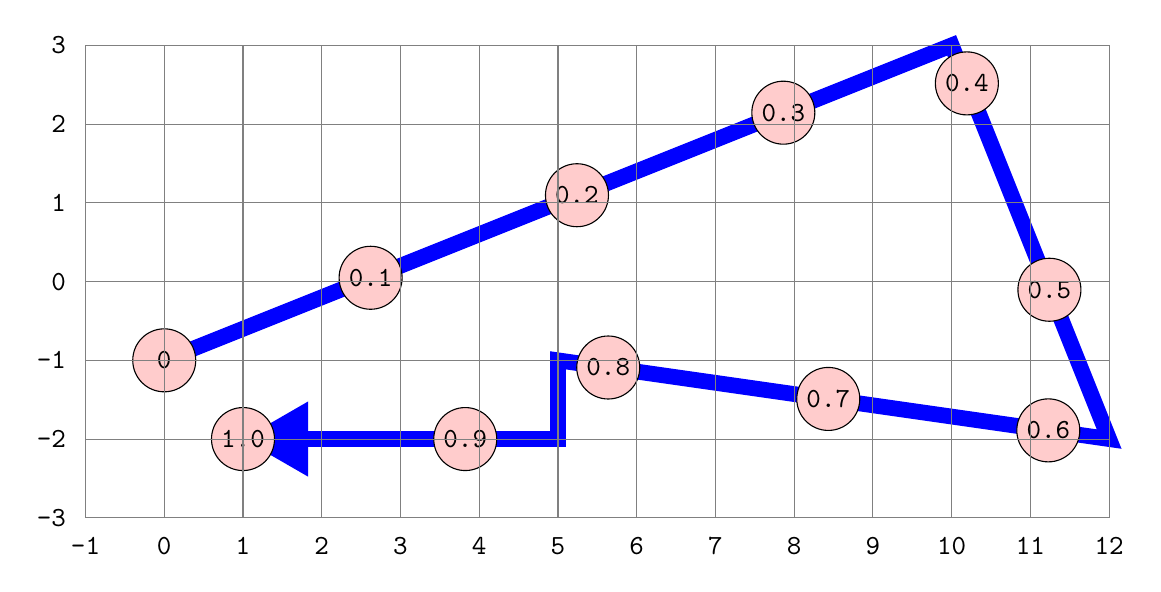
\begin{tikzpicture}
\draw[line width=0.2cm,blue,->,>=triangle 60] (0,-1) -- (10,3) -- (12,-2) -- (5,-1) -- (5,-2) -- (1,-2);
\fill[blue] (0, -1) circle (0);

\draw[blue] (0, -1)
circle (0.0);
\fill[red!20] (0.0, -1.0) circle (0.4);

\draw[black] (0.0, -1.0)
circle (0.4);
\draw (0.0, -1.0) node[color=black] {{\texttt{0}}};\fill[red!20] (2.62077050974, 0.0483082038965) circle (0.4);

\draw[black] (2.62077050974, 0.0483082038965)
circle (0.4);
\draw (2.62077050974, 0.0483082038965) node[color=black] {{\texttt{0.1}}};\fill[red!20] (5.24154101948, 1.09661640779) circle (0.4);

\draw[black] (5.24154101948, 1.09661640779)
circle (0.4);
\draw (5.24154101948, 1.09661640779) node[color=black] {{\texttt{0.2}}};\fill[red!20] (7.86231152922, 2.14492461169) circle (0.4);

\draw[black] (7.86231152922, 2.14492461169)
circle (0.4);
\draw (7.86231152922, 2.14492461169) node[color=black] {{\texttt{0.3}}};\fill[red!20] (10.1932328156, 2.51691796104) circle (0.4);

\draw[black] (10.1932328156, 2.51691796104)
circle (0.4);
\draw (10.1932328156, 2.51691796104) node[color=black] {{\texttt{0.4}}};\fill[red!20] (11.2415410195, -0.103852548706) circle (0.4);

\draw[black] (11.2415410195, -0.103852548706)
circle (0.4);
\draw (11.2415410195, -0.103852548706) node[color=black] {{\texttt{0.5}}};\fill[red!20] (11.2274009279, -1.88962870399) circle (0.4);

\draw[black] (11.2274009279, -1.88962870399)
circle (0.4);
\draw (11.2274009279, -1.88962870399) node[color=black] {{\texttt{0.6}}};\fill[red!20] (8.43311382888, -1.4904448327) circle (0.4);

\draw[black] (8.43311382888, -1.4904448327)
circle (0.4);
\draw (8.43311382888, -1.4904448327) node[color=black] {{\texttt{0.7}}};\fill[red!20] (5.63882672982, -1.0912609614) circle (0.4);

\draw[black] (5.63882672982, -1.0912609614)
circle (0.4);
\draw (5.63882672982, -1.0912609614) node[color=black] {{\texttt{0.8}}};\fill[red!20] (3.82265622333, -2.0) circle (0.4);

\draw[black] (3.82265622333, -2.0)
circle (0.4);
\draw (3.82265622333, -2.0) node[color=black] {{\texttt{0.9}}};\fill[red!20] (1.0, -2.0) circle (0.4);

\draw[black] (1.0, -2.0)
circle (0.4);
\draw (1.0, -2.0) node[color=black] {{\texttt{1.0}}};\draw[gray] (-1.0,-3.0) -- (-1.0,3);
\draw[gray] (0.0,-3.0) -- (0.0,3);
\draw[gray] (1.0,-3.0) -- (1.0,3);
\draw[gray] (2.0,-3.0) -- (2.0,3);
\draw[gray] (3.0,-3.0) -- (3.0,3);
\draw[gray] (4.0,-3.0) -- (4.0,3);
\draw[gray] (5.0,-3.0) -- (5.0,3);
\draw[gray] (6.0,-3.0) -- (6.0,3);
\draw[gray] (7.0,-3.0) -- (7.0,3);
\draw[gray] (8.0,-3.0) -- (8.0,3);
\draw[gray] (9.0,-3.0) -- (9.0,3);
\draw[gray] (10.0,-3.0) -- (10.0,3);
\draw[gray] (11.0,-3.0) -- (11.0,3);
\draw[gray] (12.0,-3.0) -- (12.0,3);
\draw[gray] (-1.0,-3.0) -- (12,-3.0);
\draw[gray] (-1.0,-2.0) -- (12,-2.0);
\draw[gray] (-1.0,-1.0) -- (12,-1.0);
\draw[gray] (-1.0,0.0) -- (12,0.0);
\draw[gray] (-1.0,1.0) -- (12,1.0);
\draw[gray] (-1.0,2.0) -- (12,2.0);
\draw[gray] (-1.0,3.0) -- (12,3.0);
\draw(-1, -3) node [font=\ttfamily, label=below:{\texttt{-1}}] {};
\draw(0, -3) node [font=\ttfamily, label=below:{\texttt{0}}] {};
\draw(1, -3) node [font=\ttfamily, label=below:{\texttt{1}}] {};
\draw(2, -3) node [font=\ttfamily, label=below:{\texttt{2}}] {};
\draw(3, -3) node [font=\ttfamily, label=below:{\texttt{3}}] {};
\draw(4, -3) node [font=\ttfamily, label=below:{\texttt{4}}] {};
\draw(5, -3) node [font=\ttfamily, label=below:{\texttt{5}}] {};
\draw(6, -3) node [font=\ttfamily, label=below:{\texttt{6}}] {};
\draw(7, -3) node [font=\ttfamily, label=below:{\texttt{7}}] {};
\draw(8, -3) node [font=\ttfamily, label=below:{\texttt{8}}] {};
\draw(9, -3) node [font=\ttfamily, label=below:{\texttt{9}}] {};
\draw(10, -3) node [font=\ttfamily, label=below:{\texttt{10}}] {};
\draw(11, -3) node [font=\ttfamily, label=below:{\texttt{11}}] {};
\draw(12, -3) node [font=\ttfamily, label=below:{\texttt{12}}] {};
\draw(-1, -3) node [font=\ttfamily, label=left:{\texttt{-3}}] {};
\draw(-1, -2) node [font=\ttfamily, label=left:{\texttt{-2}}] {};
\draw(-1, -1) node [font=\ttfamily, label=left:{\texttt{-1}}] {};
\draw(-1, 0) node [font=\ttfamily, label=left:{\texttt{0}}] {};
\draw(-1, 1) node [font=\ttfamily, label=left:{\texttt{1}}] {};
\draw(-1, 2) node [font=\ttfamily, label=left:{\texttt{2}}] {};
\draw(-1, 3) node [font=\ttfamily, label=left:{\texttt{3}}] {};
\end{tikzpicture}

\end{center}

\end{document}
